\notechapter{N-20260318}{Matrix Computation III: Canonical Forms, Spectral Localization, and Eigenvalue Iteration}

\section{Before computing an eigenvalue, decide what can change}

A matrix changes when the basis changes.  If
\[
  B=S^{-1}AS,
\]
then the entries of \(B\) may look nothing like those of \(A\), yet both matrices represent the same linear operator in different coordinates.  A useful theory of eigenvalues therefore begins by separating coordinate accidents from invariant structure.

Three questions guide this chapter.

First, what algebraic data survive every change of basis?  Canonical forms answer this.  Second, before carrying out an expensive computation, where can the eigenvalues possibly lie?  Gershgorin's theorem gives a cheap geometric answer.  Third, once a spectral region or dominant mode has been identified, how can one actually approximate the corresponding eigenvector?  Power and inverse iterations turn localization into computation.

These are different levels of information:
\[
  \text{canonical structure}
  \longrightarrow
  \text{spectral localization}
  \longrightarrow
  \text{numerical approximation}.
\]
Trying to use one level as a substitute for another causes confusion.  Jordan form explains exact structure but is usually a poor numerical algorithm.  Gershgorin discs are robust and cheap but rarely exact.  Iteration computes selected eigenpairs but only under separation and stability assumptions.

\section{The polynomial matrix \texorpdfstring{$\lambda I-A$}{lambda I minus A} contains more than the characteristic polynomial}

The characteristic polynomial
\[
  \chi_A(\lambda)=\det(\lambda I-A)
\]
records the eigenvalues with algebraic multiplicity.  It does not, by itself, reveal how many Jordan blocks occur or how large they are.  That missing information is already present in the whole polynomial matrix
\[
  \lambda I-A,
\]
not merely in its determinant.

Work over the principal ideal domain \(\mathbb C[\lambda]\).  Row and column operations are allowed when they are invertible over this ring: exchange two rows or columns, add a polynomial multiple of one to another, or multiply by a nonzero constant.  These operations produce polynomial matrices
\[
  U(\lambda)(\lambda I-A)V(\lambda)
\]
with unimodular \(U,V\), meaning their determinants are nonzero constants.

Every polynomial matrix of rank \(r\) can be reduced to Smith normal form
\[
  \operatorname{diag}
  \bigl(d_1(\lambda),\ldots,d_r(\lambda),0,\ldots,0\bigr),
\]
where the nonzero polynomials are monic and satisfy
\[
  d_1\mid d_2\mid\cdots\mid d_r.
\]
The polynomials \(d_i\) are the invariant factors.

If \(D_k(\lambda)\) denotes the monic greatest common divisor of all nonzero \(k\times k\) minors, then
\[
  d_1=D_1,
  \qquad
  d_k=\frac{D_k}{D_{k-1}}.
\]
The determinant is only the last determinantal divisor:
\[
  D_n=d_1d_2\cdots d_n=\chi_A(\lambda).
\]
The smaller minors are what remember how the characteristic polynomial is distributed among cyclic pieces.

\section{Invariant factors are a module decomposition}

Let \(V=\mathbb C^n\), and let the indeterminate \(\lambda\) act on vectors by
\[
  \lambda\cdot v=Av.
\]
This turns \(V\) into a \(\mathbb C[\lambda]\)-module.  The structure theorem for finitely generated modules over a principal ideal domain gives
\[
  V
  \cong
  \bigoplus_i
  \mathbb C[\lambda]/(d_i(\lambda)),
\]
where the nonconstant invariant factors are those of \(\lambda I-A\).

This description explains why Smith form belongs naturally beside canonical matrix forms.  A cyclic summand
\[
  \mathbb C[\lambda]/(d(\lambda))
\]
is generated by one vector
\[
  v,Av,A^2v,\ldots,
\]
subject to the relation \(d(A)v=0\).  In a suitable cyclic basis, the matrix of \(A\) on this summand is the companion matrix of \(d\).  Taking the direct sum over invariant factors gives the rational canonical form.

The largest invariant factor is the minimal polynomial:
\[
  m_A(\lambda)=d_n(\lambda),
\]
while their product is the characteristic polynomial.  Thus
\[
  m_A\mid\chi_A.
\]
The minimal polynomial records the strongest polynomial relation satisfied by the operator and controls every polynomial expression in \(A\), including high powers and matrix functions.

\section{From invariant factors to Jordan blocks}

Over \(\mathbb C\), factor each invariant factor into powers of linear terms.  The resulting powers
\[
  (\lambda-\mu)^s
\]
are called elementary divisors.  Each elementary divisor corresponds to one Jordan block
\[
  J_s(\mu).
\]

For example, suppose the elementary divisors are
\[
  (\lambda-2)^2,
  \qquad
  (\lambda-2),
  \qquad
  (\lambda-3).
\]
Then the Jordan form is
\[
  J_2(2)\oplus J_1(2)\oplus J_1(3).
\]
The characteristic polynomial is
\[
  (\lambda-2)^3(\lambda-3),
\]
but the minimal polynomial is only
\[
  (\lambda-2)^2(\lambda-3).
\]
The exponent \(2\) of \(\lambda-2\) in the minimal polynomial records the largest Jordan block for eigenvalue \(2\), not the total multiplicity of that eigenvalue.

A concrete polynomial-matrix example makes the mechanism visible.  Let
\[
  A=
  \begin{bmatrix}
    2&1&0\\
    0&2&0\\
    0&0&3
  \end{bmatrix}.
\]
Then
\[
  \lambda I-A=
  \begin{bmatrix}
    \lambda-2&-1&0\\
    0&\lambda-2&0\\
    0&0&\lambda-3
  \end{bmatrix}.
\]
Because one entry is the unit \(-1\), the gcd of the entries is \(D_1=1\).  Among the \(2\times2\) minors appear both
\[
  (\lambda-2)^2
  \qquad\text{and}\qquad
  -(\lambda-3),
\]
whose gcd is \(1\).  Hence \(D_2=1\).  Finally,
\[
  D_3=(\lambda-2)^2(\lambda-3).
\]
The invariant factors are therefore
\[
  1,\quad1,\quad(\lambda-2)^2(\lambda-3),
\]
and the elementary divisors are
\[
  (\lambda-2)^2,\qquad(\lambda-3).
\]
They recover the block structure \(J_2(2)\oplus J_1(3)\).

\section{Jordan chains turn algebraic multiplicity into dynamics}

A Jordan chain for eigenvalue \(\mu\) is a sequence
\[
  v_1,v_2,\ldots,v_s
\]
satisfying
\[
  (A-\mu I)v_1=0,
\]
\[
  (A-\mu I)v_{j+1}=v_j.
\]
The first vector is an eigenvector; the others are generalized eigenvectors.  In this basis the operator acts by
\[
  Av_1=\mu v_1,
  \qquad
  Av_{j+1}=\mu v_{j+1}+v_j.
\]

Write a Jordan block as
\[
  J=\mu I+N,
  \qquad N^s=0.
\]
Then
\[
  J^k
  =\sum_{j=0}^{s-1}
  \binom{k}{j}\mu^{k-j}N^j.
\]
The exponential term \(\mu^k\) is decorated by polynomial factors in \(k\).  This is the precise origin of terms such as
\[
  k\mu^{k-1},
  \qquad
  \binom{k}{2}\mu^{k-2}.
\]

For
\[
  J=
  \begin{bmatrix}
    1&1\\
    0&1
  \end{bmatrix},
\]
we obtain
\[
  J^k=
  \begin{bmatrix}
    1&k\\
    0&1
  \end{bmatrix}.
\]
Every eigenvalue equals \(1\), yet powers grow linearly.  The Jordan chain carries dynamical information that the list of eigenvalues alone cannot express.

This also explains why Jordan form is mathematically revealing but numerically delicate.  A tiny perturbation can split a multiple eigenvalue and destroy a large Jordan block.  Computing exact block sizes from floating-point data is therefore ill-conditioned.  Stable numerical algorithms usually prefer Schur form,
\[
  A=QTQ^*,
\]
where \(Q\) is unitary and \(T\) is upper triangular.  The diagonal of \(T\) gives the eigenvalues while unitary similarity avoids an ill-conditioned eigenvector basis.

\section{Gershgorin reads spectral information directly from rows}

Canonical forms describe exact similarity invariants, but they are not a cheap first diagnostic.  Gershgorin's theorem locates every eigenvalue using only row sums.

For \(A=(a_{ij})\), define
\[
  R_i=\sum_{j\ne i}|a_{ij}|.
\]
The \(i\)-th Gershgorin disc is
\[
  G_i=\{z\in\mathbb C:|z-a_{ii}|\le R_i\}.
\]
Every eigenvalue lies in
\[
  \bigcup_iG_i.
\]

The proof is a one-line maximum-coordinate argument.  If
\[
  Ax=\lambda x
\]
and \(|x_i|=\max_j|x_j|\), then
\[
  (\lambda-a_{ii})x_i
  =\sum_{j\ne i}a_{ij}x_j.
\]
Therefore
\[
  |\lambda-a_{ii}|
  \le
  \sum_{j\ne i}|a_{ij}|
  \frac{|x_j|}{|x_i|}
  \le R_i.
\]
The chosen coordinate may depend on the eigenvector, so the theorem gives a union of discs rather than one fixed disc.

\begin{figure}[H]
\centering
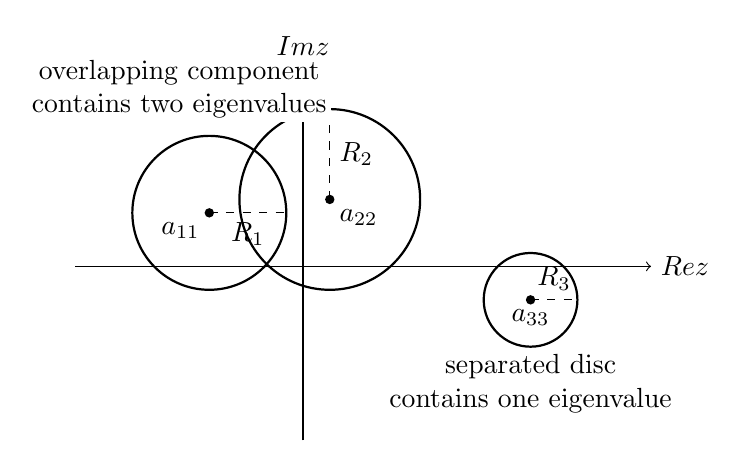
\begin{tikzpicture}[scale=0.85]
  \draw[->] (-3.4,0) -- (5.2,0) node[right] {$\operatorname{Re}z$};
  \draw[->] (0,-2.6) -- (0,3.0) node[above] {$\operatorname{Im}z$};
  \coordinate (c1) at (-1.4,0.8);
  \coordinate (c2) at (0.4,1.0);
  \coordinate (c3) at (3.4,-0.5);
  \draw[thick] (c1) circle (1.15);
  \draw[thick] (c2) circle (1.35);
  \draw[thick] (c3) circle (0.7);
  \fill (c1) circle (2pt) node[below left] {$a_{11}$};
  \fill (c2) circle (2pt) node[below right] {$a_{22}$};
  \fill (c3) circle (2pt) node[below] {$a_{33}$};
  \draw[dashed] (c1) -- ++(1.15,0) node[midway,below] {$R_1$};
  \draw[dashed] (c2) -- ++(0,1.35) node[midway,right] {$R_2$};
  \draw[dashed] (c3) -- ++(0.7,0) node[midway,above] {$R_3$};
  \node[align=center,fill=white,inner sep=1.5pt] at (-1.85,2.65)
    {overlapping component\\contains two eigenvalues};
  \node[align=center] at (3.4,-1.75) {separated disc\\contains one eigenvalue};
\end{tikzpicture}
\caption{A separated component containing exactly $m$ Gershgorin discs contains exactly $m$ eigenvalues, counted with algebraic multiplicity.}
\end{figure}

\section{Separated discs count eigenvalues, not merely contain them}

A stronger form of the theorem says that if a connected component of
\[
  \bigcup_iG_i
\]
contains exactly \(m\) discs and is disjoint from the remaining discs, then it contains exactly \(m\) eigenvalues, counted with algebraic multiplicity.

The idea is deformation.  Consider matrices
\[
  A(t)=D+t(A-D),
  \qquad 0\le t\le1,
\]
where \(D\) is the diagonal part of \(A\).  At \(t=0\), every eigenvalue is a diagonal entry, and each disc has radius zero.  As \(t\) increases, the discs expand continuously.  If one cluster stays separated from the rest, eigenvalues cannot cross the gap between components.  The number inside that component is therefore conserved.

For example, let
\[
  A=
  \begin{bmatrix}
    4&1&0\\
    1&4&0\\
    0&0&9
  \end{bmatrix}.
\]
The first two discs are both the interval-like discs centered at \(4\) with radius \(1\), while the third is the point \(9\).  Hence two eigenvalues lie in the component around \(4\), and one lies at \(9\).  Direct calculation gives
\[
  \sigma(A)=\{3,5,9\},
\]
exactly matching the count.

This separated-component principle is particularly useful for proving that a matrix is nonsingular.  If every Gershgorin disc avoids the origin, then \(0\notin\sigma(A)\).  Strict diagonal dominance is the familiar special case
\[
  |a_{ii}|>\sum_{j\ne i}|a_{ij}|.
\]

\section{Diagonal scaling can reveal localization hidden by coordinates}

Gershgorin discs depend on the chosen basis even though eigenvalues do not.  This is not a defect; it is an opportunity.  A diagonal similarity
\[
  B=D^{-1}AD
\]
preserves the spectrum while changing off-diagonal magnitudes:
\[
  b_{ij}=d_i^{-1}a_{ij}d_j.
\]

Consider
\[
  A=
  \begin{bmatrix}
    1&100\\
    0.01&2
  \end{bmatrix}.
\]
The row discs have radii \(100\) and \(0.01\), giving a very poor picture.  Choose
\[
  D=
  \begin{bmatrix}
    100&0\\
    0&1
  \end{bmatrix}.
\]
Then
\[
  D^{-1}AD
  =
  \begin{bmatrix}
    1&1\\
    1&2
  \end{bmatrix}.
\]
Now both radii are \(1\).  The eigenvalues have not moved, but the coordinates have been balanced so that the row equations display their coupling more honestly.

Choosing an optimal diagonal scaling is itself a nontrivial problem.  The example nonetheless illustrates a broad numerical principle: poor coordinates can hide useful structure, and similarity transformations can expose it without changing the underlying operator.

\section{Power iteration extracts a dominant direction}

Suppose \(A\) is diagonalizable with eigenpairs \((\lambda_i,v_i)\), ordered so that
\[
  |\lambda_1|>|\lambda_2|\ge\cdots.
\]
Write the initial vector as
\[
  x_0=c_1v_1+c_2v_2+\cdots+c_nv_n,
  \qquad c_1\ne0.
\]
Then
\[
  A^kx_0
  =\lambda_1^k
  \left(
    c_1v_1+\sum_{j\ge2}c_j
    \left(\frac{\lambda_j}{\lambda_1}\right)^kv_j
  \right).
\]
After normalization, the smaller ratios decay, so the direction approaches \(v_1\).  The asymptotic rate is governed by
\[
  \left|\frac{\lambda_2}{\lambda_1}\right|.
\]

Take
\[
  A=
  \begin{bmatrix}
    2&1\\
    1&2
  \end{bmatrix}.
\]
Its eigenvectors are
\[
  v_1=\begin{bmatrix}1\\1\end{bmatrix},
  \qquad
  v_2=\begin{bmatrix}1\\-1\end{bmatrix},
\]
with eigenvalues \(3\) and \(1\).  Starting from
\[
  x_0=\begin{bmatrix}1\\0\end{bmatrix}
  =\frac12v_1+\frac12v_2,
\]
we obtain
\[
  A^kx_0
  =\frac12
  \begin{bmatrix}
    3^k+1\\
    3^k-1
  \end{bmatrix}.
\]
The ratio of the two coordinates tends to \(1\), and the normalized vector approaches the dominant direction \((1,1)^T\).

A convenient eigenvalue estimate is the Rayleigh quotient
\[
  \rho(x)=\frac{x^*Ax}{x^*x}.
\]
For Hermitian \(A\), if \(x_k\) approaches a normalized eigenvector, then \(\rho(x_k)\) approaches its eigenvalue.  The residual
\[
  r_k=Ax_k-\rho(x_k)x_k
\]
provides an a posteriori check: an exact eigenvector has zero residual.

\section{Power iteration has precise failure modes}

The method is not guaranteed merely because a matrix has eigenvalues.

If the initial vector has no component in the dominant eigenspace, the dominant mode never appears.  If two eigenvalues tie in modulus, the direction may fail to converge.  For example,
\[
  A=
  \begin{bmatrix}
    1&0\\
    0&-1
  \end{bmatrix}
\]
has two eigenvalues of equal modulus.  Starting from a generic vector, the second coordinate changes sign at every step, so the normalized sequence oscillates.

Nonnormality creates another complication.  Even when one eigenvalue is asymptotically dominant, an ill-conditioned eigenvector basis can produce large transient mixtures before the asymptotic regime becomes visible.  A small residual is therefore more informative than a visually stable sequence of normalized coordinates.

Finally, normalization prevents overflow but does not repair loss of information.  If roundoff repeatedly suppresses a weak component or if the dominant eigenvalue is poorly separated, convergence may stagnate.

\section{Inverse iteration turns a target into a dominant mode}

Power iteration naturally finds the eigenvalue of largest modulus.  To find an eigenvalue near a chosen shift \(\mu\), apply power iteration to
\[
  (A-\mu I)^{-1}.
\]
Its eigenvalues are
\[
  \frac1{\lambda_j-\mu}.
\]
The eigenvalue of \(A\) closest to \(\mu\) becomes the dominant eigenvalue of the inverse operator.

The practical iteration is not to form the inverse.  Instead, solve
\[
  (A-\mu I)y_{k+1}=x_k
\]
and normalize
\[
  x_{k+1}=\frac{y_{k+1}}{\|y_{k+1}\|}.
\]
If the shift stays fixed, factor \(A-\mu I\) once and reuse the triangular solves.  This makes shifted inverse iteration efficient when several steps are required.

The apparent paradox is that the method becomes stronger as \(\mu\) approaches an eigenvalue, while the linear system becomes more ill-conditioned.  The near singularity is exactly what amplifies the desired eigendirection.  Stable pivoting, residual monitoring, and an appropriate stopping criterion are therefore essential.

\section{Rayleigh quotient iteration lets the shift move}

A natural refinement updates the shift using the current Rayleigh quotient:
\[
  \mu_k=\frac{x_k^*Ax_k}{x_k^*x_k},
\]
then solves
\[
  (A-\mu_kI)y_{k+1}=x_k
\]
and normalizes.

For Hermitian matrices and a sufficiently good initial vector, Rayleigh quotient iteration converges cubically.  This remarkable speed comes from two facts: the Rayleigh quotient already approximates the eigenvalue to second order in the angular error, and inverse iteration strongly amplifies the nearest eigendirection.

Take again
\[
  A=
  \begin{bmatrix}
    2&1\\
    1&2
  \end{bmatrix}.
\]
If
\[
  x_0=\frac1{\sqrt5}
  \begin{bmatrix}2\\1\end{bmatrix},
\]
then
\[
  \mu_0=x_0^TAx_0=\frac{14}{5}=2.8,
\]
already close to the dominant eigenvalue \(3\).  Solving with \(A-2.8I\) strongly favors the \((1,1)^T\) direction, and the next Rayleigh quotient is dramatically more accurate.

The method should not be described as universally cubic.  Symmetry or normality, a nearby simple eigenvalue, and a sufficiently accurate starting vector are important.  For a general nonnormal matrix, convergence can be less regular and the moving linear systems can become difficult.

\section{Large matrices lead from vectors to Krylov subspaces}

Power iteration uses the one-dimensional space spanned by the newest vector.  A more informative approach retains the whole Krylov space
\[
  \mathcal K_k(A,x_0)
  =\operatorname{span}
  \{x_0,Ax_0,\ldots,A^{k-1}x_0\}.
\]
Instead of asking one vector to represent all spectral information, project \(A\) onto this growing subspace.

For Hermitian matrices, the Lanczos process constructs an orthonormal basis of the Krylov space and produces a small tridiagonal matrix.  Its eigenvalues, called Ritz values, approximate selected eigenvalues of \(A\).  For general matrices, Arnoldi iteration produces an upper Hessenberg projection.

These methods are the large-scale descendants of power iteration.  They retain the same polynomial idea---vectors in \(\mathcal K_k\) have the form \(p_{k-1}(A)x_0\)---but optimize over many polynomials rather than repeatedly using only \(p(t)=t^k\).  This is why Krylov eigensolvers can resolve several eigenvalues and converge much faster than plain power iteration.

\section{The three viewpoints should remain distinct}

Smith form and invariant factors answer what survives exact algebraic equivalence.  Jordan chains explain generalized eigenvectors, polynomial factors in powers, and the minimal polynomial.  Schur form is usually the numerically stable replacement when floating-point computation is required.

Gershgorin discs answer a cheaper question: where can the spectrum lie, and can separated clusters be counted before computing them?  Diagonal scaling shows that localization may improve after a better choice of coordinates.

Power iteration, shifted inverse iteration, and Rayleigh quotient iteration answer a computational question: how can a selected eigendirection be amplified?  Their success depends on spectral separation, a nonzero starting component, stable linear solves, and residual checks.  Krylov methods generalize the same idea from one direction to an adaptively constructed subspace.

The natural workflow is therefore
\[
\begin{gathered}
  \text{understand invariant structure}\\
  \big\downarrow\\
  \text{localize the spectrum}\\
  \big\downarrow\\
  \text{choose and verify an iteration}.
\end{gathered}
\]
Canonical forms tell us what the operator is.  Localization tells us where to look.  Iteration tells us how to reach the part we want.
